%!TEX root = ../main.tex

%
% Notes: 
%
%  exact implementation
%  comparison with rollback at batch N
%  relaxing the solvers
%  dealing with false positives
%
%  running on TPC-C/sanjay's.  equality is easier
%
% Need names for
%  * rollback
%  * exact solution
%  * fixing an individual/batch of queries
%
\section{Experiments}
\label{sec:experiments}


  \begin{figure*}[h]
  \hspace*{-.1in}
  \centering
    \vspace*{-.2in}
    \begin{subfigure}[t]{.33\textwidth}
    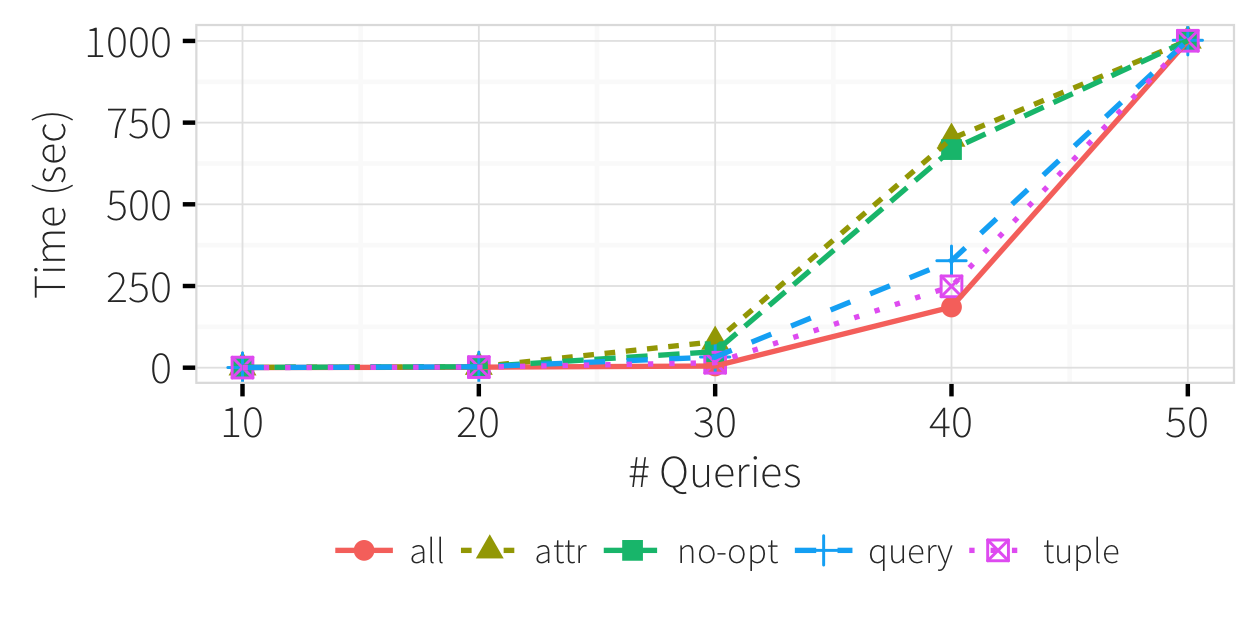
\includegraphics[width = .99\columnwidth]{figures/multi_time}
    \vspace*{-.25in}
    \caption{Performance for multiple corruptions.}
    \label{f:multi_time} 
    \end{subfigure}
    \begin{subfigure}[t]{.33\textwidth}
    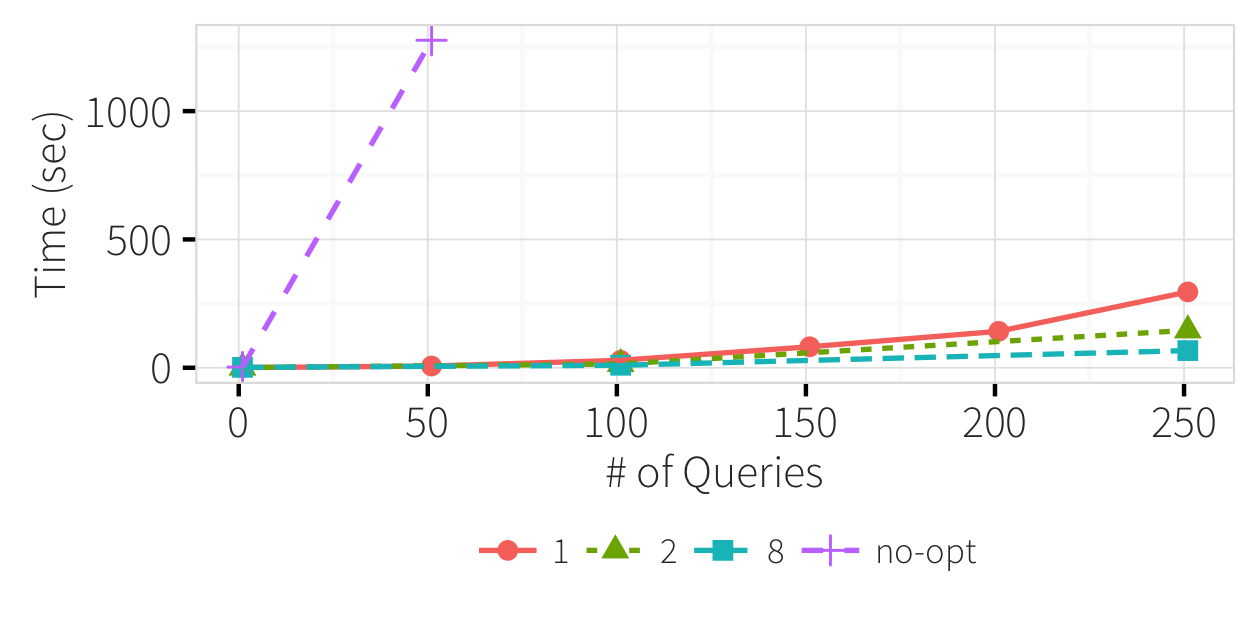
\includegraphics[width = .99\columnwidth]{figures/incrementalcompare_time}
    \vspace*{-.25in}
    \caption{Performance for single corruption.}
    \label{f:singlequeryinc_time} 
    \end{subfigure}
    \begin{subfigure}[t]{.33\textwidth}
    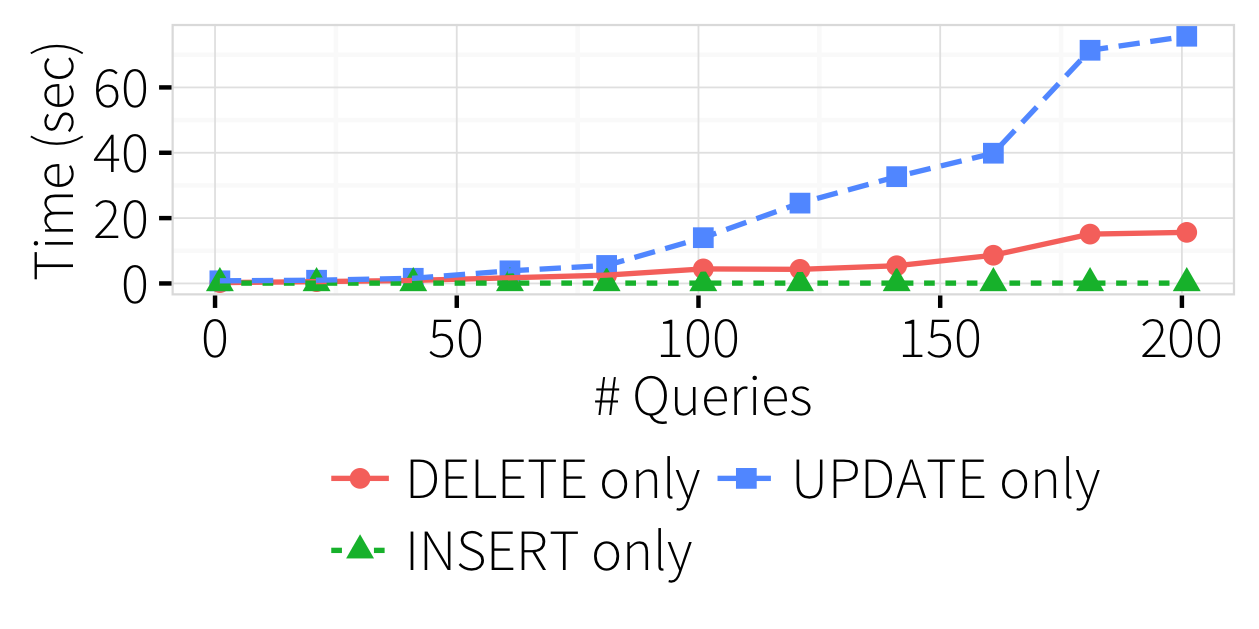
\includegraphics[width = .99\columnwidth]{figures/indelup_time}
    \vspace*{-.25in}
    \caption{Performance for different query types.}
    \label{f:indelup_time} 
    \end{subfigure}
    \vspace*{0.2in}
    \\
    \hspace*{-.1in}
    \begin{subfigure}[t]{.33\textwidth}
    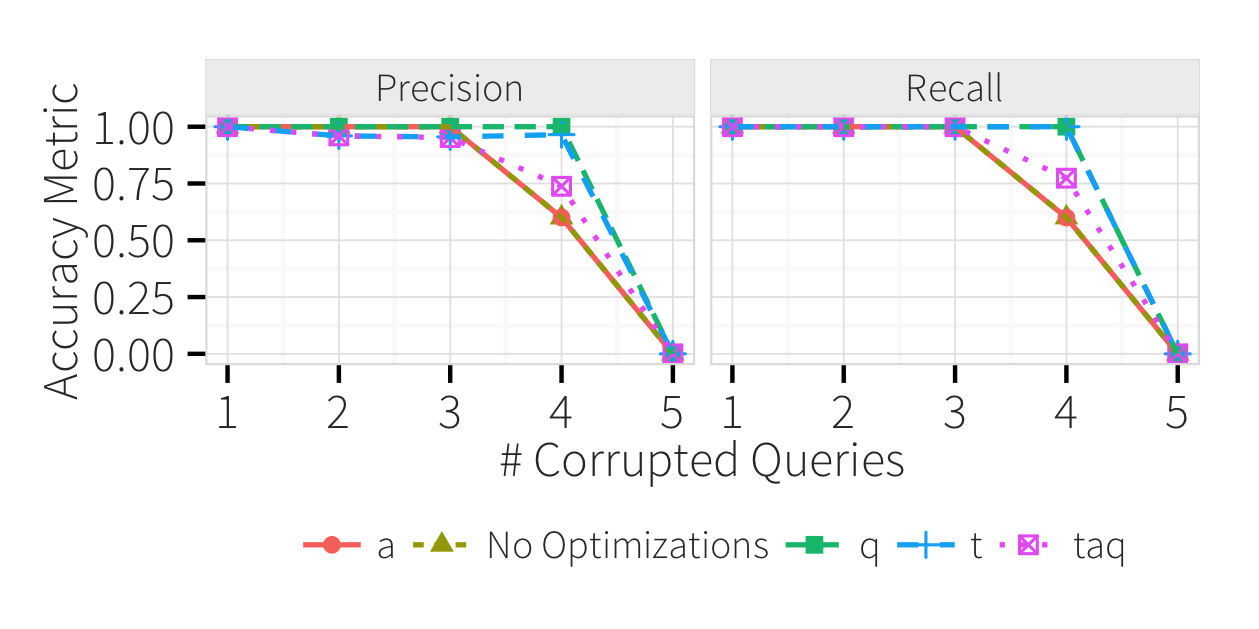
\includegraphics[width = .99\columnwidth]{figures/multi_pr}
    \vspace*{-.25in}
    \caption{Accuracy for multiple corruptions.}
    \label{f:multi_acc} 
    \end{subfigure}
    \begin{subfigure}[t]{.33\textwidth}
    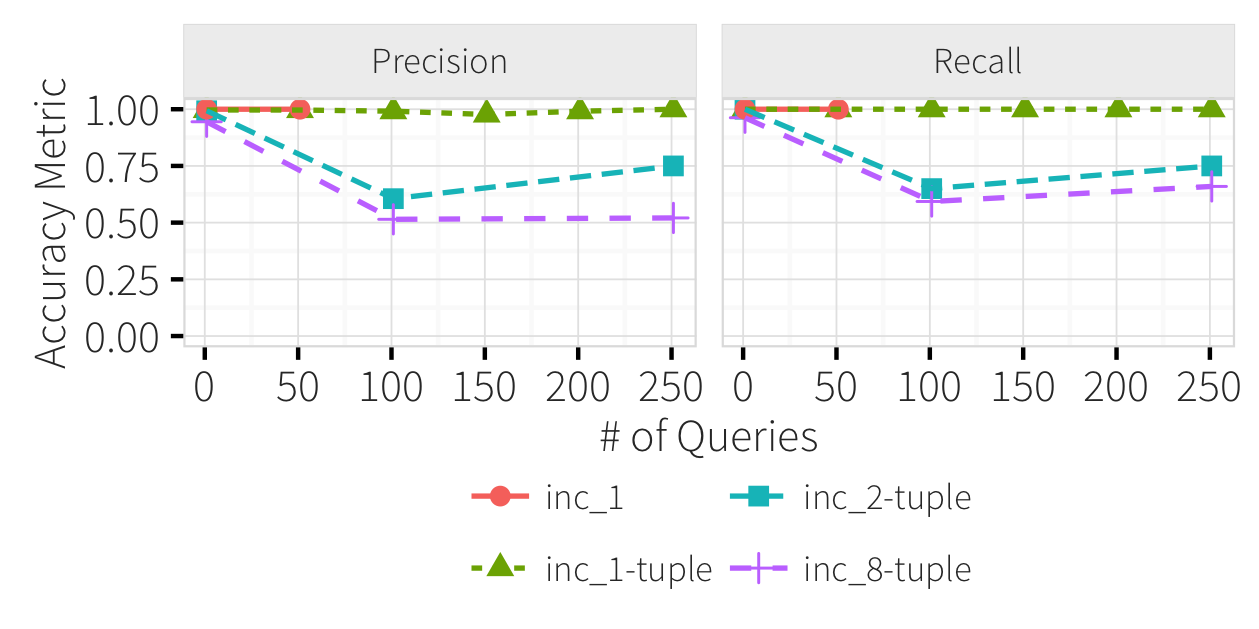
\includegraphics[width = .99\columnwidth]{figures/incrementalcompare_acc}
    \vspace*{-.25in}
    \caption{Accuracy for single corruption.}
    \label{f:singlequeryinc_acc} 
    \end{subfigure}
    \begin{subfigure}[t]{.33\textwidth}
    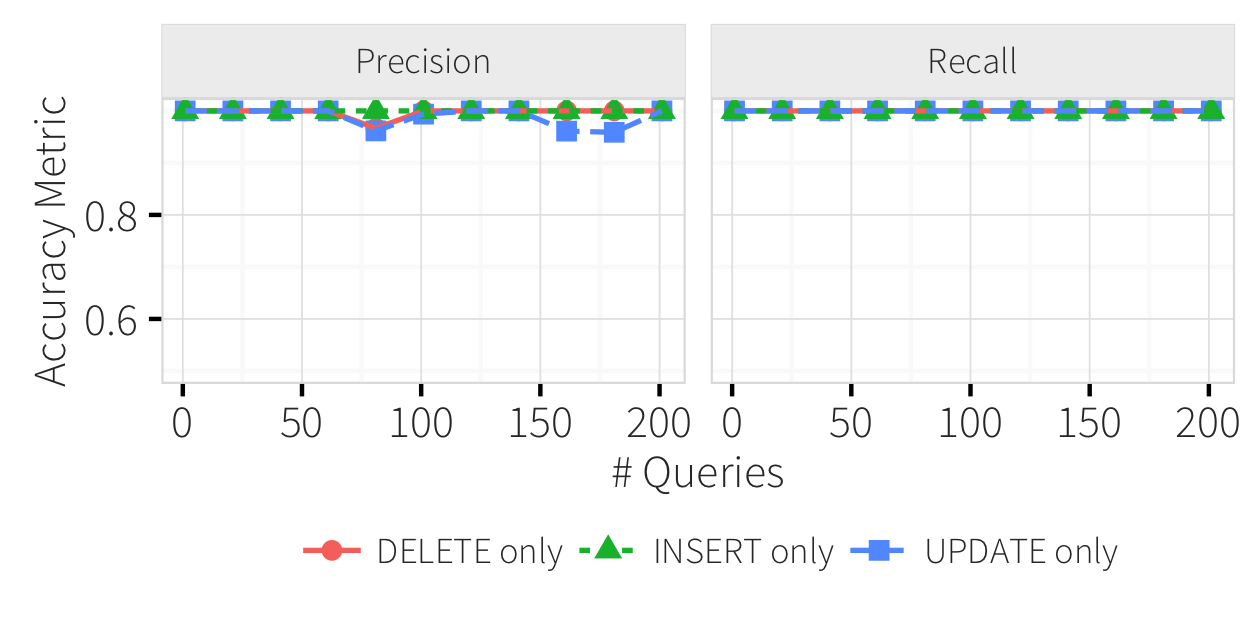
\includegraphics[width = .99\columnwidth]{figures/indelup_pr}
    \vspace*{-.25in}
    \caption{Accuracy for different query types.}
    \label{f:indelup_acc} 
    \end{subfigure}
    \vspace*{-.1in}
    \caption{Preliminary experiments.}
    \vspace*{-.15in}
  \end{figure*}


In this section, we carefully study the performance and accuracy
characteristics of the basic MILP-based repair algorithm, 
slicing-based optimizations that improve the latency of the system, 
and the incremental algorithm for single query corruptions. 
%and 
%the multi-pass tuple-slicing algorithm that tolerates incomplete complaint sets with minimal loss in accuracy.
Our goal is to understand these trade-offs in
controlled synthetic scenarios, as well as study the effectiveness
in typical database query workloads based on widely used benchmarks.
% \xlw{ By default, we set \sys as the incremental approach with tuple slicing optimization ($inc_1-tuple$) as it fixes our default synthetic query logs and benchmark workloads with minimum time cost and near perfect accuracy.  }


To this end, our experiments are organized as follows: First, 
we compare the basic and incremental MILP algorithm against the different optimizations 
to highlight the value of different optimizations and the limitatios of the basic approach.  
We then compare the repair costs of \texttt{INSERT}, \texttt{DELETE}, or \texttt{UPDATE}-only query logs 
and find that the latter query type is by far the most complicated and costly to repair.
For the subsequent experiments, we focus solely on \texttt{UPDATE}-only synthetic workloads 
to understand how \sys responds to different query logs and databases.  
We end with an evaluation using established database transaction benchmarks from OLTP-bench~\cite{difallah2013oltp},
TPC-C~\cite{tpcc} and TATP~\cite{tatp}. 
All experiments were run on 12x2.66 GHz  machines with 16GB RAM running CentOS release 6.6. And we use IBM CPLEX~\cite{cplex2014v12} 
as the MILP solver.



% establish the quality limitations of existing heuristics and the need for a formal, 
% constraint-based algorithm (\exact).  Second, we study how each of the 
% optimizations described in Section~\ref{s:optimiztaions} improves algorithm scalability.
% Third, we introduce different forms of error in the input complaint sets and study the 
% effectiveness of our noise-handling heuristics.  




%
% NOTE: figures are named <experimentsection>_<subsection>_<xaxis>.pdf
%

\subsection{Experimental Setup}


\iffalse
\begin{table}[t]\small
  \centering
  \begin{tabular}{@{}cll@{}}
  \toprule
  {\bf Param} & {\bf Description} & {\bf Default} \\ \midrule
  $V_d$  & Domain range of the attributes  & $[0, 100]$ \\
  $N_D$  & \# tuples in final database & $1000$ \\
  $N_a$  & \# attributes in database & $10$ \\
  $N_w$  & \# predicates in \texttt{WHERE} clauses & $1$ \\
  $N_s$  & \# \texttt{SET} clauses & $1$ \\
  $N_q$  & \# queries in query log & $300$ \\
  $idx$  & Index of corrupted query & $\{0, 25, 50,$ \\
         & (backwards from most recent) & $100, 200, 250 \}$ \\ %$\frac{N_q}{2}$ \\
  $r$    & Range size of \texttt{UPDATE} queries & 8 (tuples) \\
  $s$    & Zipf $\alpha$ param of query attributes, & $1$ \\ \bottomrule \end{tabular}
  %$set$  & Constant vs relative \texttt{SET} clauses. & const \\ 
         %& power low distribution $P(v) = v^{-s}$ & \\\end{tabular}
  \caption{Experimental Parameters}
  \label{t:params}
\end{table}
\fi


\iffalse
  \begin{table}[t]\small
    \centering
    \begin{tabular}{@{}cl@{}}
    \toprule
    {\bf Param} & {\bf Description} \\ \midrule
    $p$ & Precision: \% of repaired tuples that are correct. \\
    $r$ & Recall: \% of full complaint set repaired.\\
    % $t_{prep}$ & Time to construct CPLEX problem \\
    % $t_{send}$ & Time to send CPLEX problem to solver \\
    % $t_{solve}$ & Time for solver to generate a solutions\\
    $t_{total}$ & End-to-end execution time \\ 
    $d_{measure}$ & \red{Some sort of distance measure} \\ \bottomrule \end{tabular}
    \caption{Metrics Compared}
    \label{t:metrics}
  \end{table}
\fi




Each of our experiments follows a similar procedure. 
We generate a sequence of queries using a synthetic query generator or 
the benchmark program, and corrupt the query log as described below. 
We then execute the original and corrupt query logs on an initial (possibly empty) database,
and perform a tuple-wise comparison between the resulting database states 
to generate a true complaint set.  
We then add noise to the complaint set by removing (partial) true complaints to simulate false negatives.
Finally, we execute the evaluated algorithms on the complaints and compare the fixed
query log with the true query log, as well as the fixed and true
final database states to measure performance and accuracy metrics.
Performance is measured as wall clock
time between submitting a complaint set and the system terminating after retrieving a valid repair.  
Accuracy is measured as repair's precision (percentage of repaired tuples that were correctly fixed), 
the recall (the percentage of the full complaint set that was repaired), 
and the F1 measure (the harmonic mean of precision and recall).
Our reported metrics are the average across 20 runs.
We describe the experimental parameters in the context of the datasets and workloads below.
%Finally, Table~\ref{t:params} summarizes the key parameters that we vary throughout our experiments.  


\subsubsection{Datasets and Workloads}


%This subsection describes the query and data generation process in greater detail.

\stitle{Synthetic:} \label{sec:syntheticgen}
We generate an initial database of $N_D$ random tuples.  
The schema contains a primary key $id$ along with $N_a$ attributes $a_1\ldots a_{N_a}$, whose values are integers picked from $[0, V_d]$ uniformly at random.
We then generate a sequence of $N_q$ queries.
The default setting for these parameters are: $N_D = 1000, N_a = 10, V_d = 200, N_q = 300$.
% ~\footnote{\scriptsize We focus on \texttt{UPDATE} only query logs because they are the {\it predominant} cost in a query log.  Experiment~\ref{sec:indelup} compares \texttt{INSERT}, \texttt{DELETE} and \texttt{UPDATE} only workloads to illustrate the difference.} 
% in the format (SET and WHERE clauses) described as below. 
% UPDATE SET X,.. WHERE Y ...


\noindent \texttt{UPDATE} queries are defined by a SET clause that assigns an attribute a $Constant$ or $Relative$ value,
and a WHERE clause can either be a $Point$ predicate on a key, or a $Range$ predicate on non-key attributes:
{\scriptsize
\begin{verbatim}
 SET Clause:                WHERE Clause:
  Constant: SET (a_i=?), ..   Point: WHERE a_j=? & ..
  Relative: SET (a_i=a_i+?)   Range: WHERE a_j in [?,?+r] & ..\end{verbatim} }
where \verb|?|$\in [0, V_d]$ is random and \verb|r| is the size of the range predicate. 
Query selectivity is by default $2\%$ (\verb|r|$=2$).
Note that a range predicate where \texttt{r = 0} is distinct from a $Point$ predicate due to the non-key attribute.
The WHERE clauses in \texttt{DELETE} queries are generated in an identical fashion, while
\texttt{INSERT} queries insert values picked uniformly at random from $V_d$.
By default, we generate \texttt{UPDATE} queries with non-key range predicates and constant set clauses.

% $X \& Y$ represents the \texttt{UPDATE} query type. $X$ represents the set clause type which can be either constant update ($Constant$) or
% relative update ($Relative$). Similarly, $Y$ represents the where clause type that can be either point update ($Point$) or
% range update ($Range$). Note that the 
% we default focus on \texttt{UPDATE} queries with non-key predicates on range(s) and constant SET clauses.
% 
% The \texttt{SET} clause sets the attribute to a random constant value in $V_d$ and 
% the \texttt{WHERE} clauses form a conjunction.  
% The $set$ parameter controls whether the \texttt{UPDATE} queries set attributes to random constant values ({\it const}),  
% or relative values ({\it rel}) by incrementing by a random, possibly negative, value.  

In addition, the skew parameter $s$ determines the distribution attributes referenced in the \texttt{WHERE} and \texttt{SET} clauses.  
Each attribute in a query is picked from either a uniform distribution when $s=0$ or a zipfian distribution with exponent $s$.
This allows our experiments to vary between a uniform distribution, where each attribute is
equally likely to be picked, and a skewed distribution where nearly all attributes are the same. 

\stitle{Benchmarks: } We use the TPC-C~\cite{tpcc} and TATP~\cite{tatp} benchmarks.
The former generates the {\it ORDER} table at scale 1 with one warehouse, and uses the queries that modify the {\it ORDER} table. 
We execute a log of 2000 queries over an initial table containing 6000 tuples.  
$1837$ queries are \texttt{INSERT}s and the rest are \texttt{UPDATE}s. 
The latter TATP workload simulates the caller location system. 
We generate a database from {\it SUBSCRIBER} table with 5000 tuples and $2000$ \texttt{UPDATE} queries.
Both setups were generated using the OLTP-bench~\cite{difallah2013oltp}. 
We introduce a single corruption, and vary corrupted query's index from the most recent query $q_N$ to $q_{N-1500}$.



\stitle{Corrupting Queries:} We corrupt query $q_i$ by replacing it with a randomly
generated query of the same type based on the procedures described above.
To standardize our procedures, we selected a fixed set of indexes $idx$
that are used in all experiments. 

% \ewu{The technical report~\cite{} describes the corruption process in more detail.} 
%Appendix~\ref{app:qidx} presents
%experiments that justify the rationale behind our selection.
% xxx
% \ewu{The technical report~\cite{} describes the corruption process in more detail.} 






% \begin{figure}[h]
% \centering
%   \begin{subfigure}[t]{\columnwidth}
%   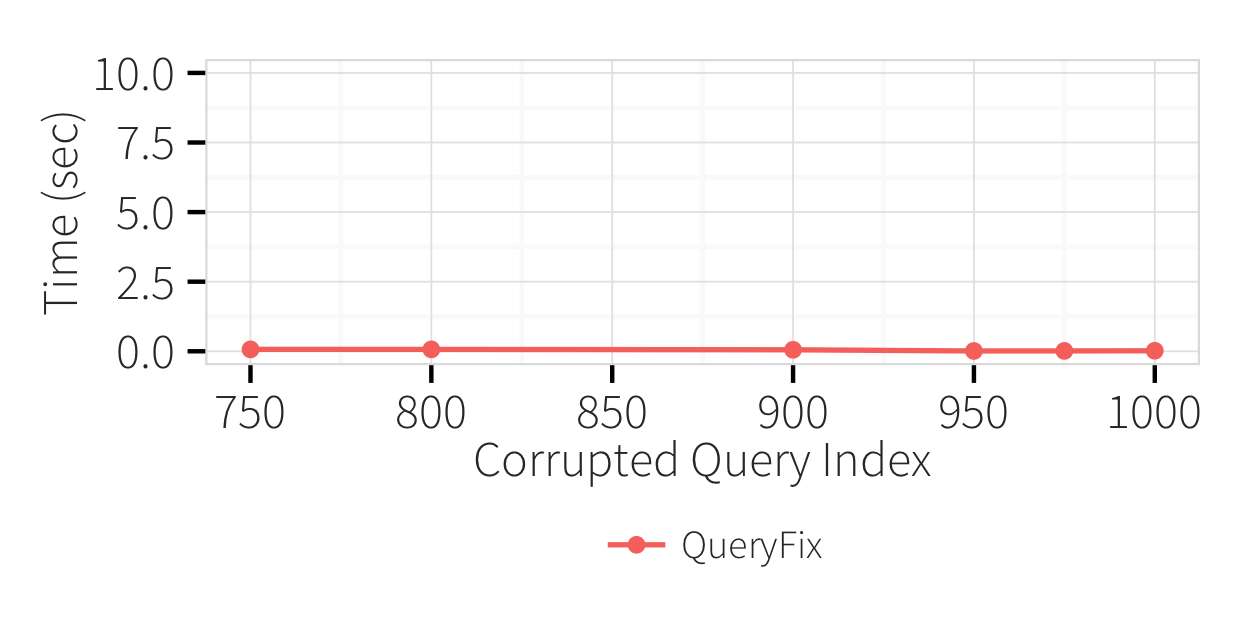
\includegraphics[width = .95\columnwidth]{figures/tpcc_time}
%   \caption{Performance on TPC-C Benchmark}
%   \label{f:tpcc} 
%   \end{subfigure}
%   \begin{subfigure}[t]{\columnwidth}
%   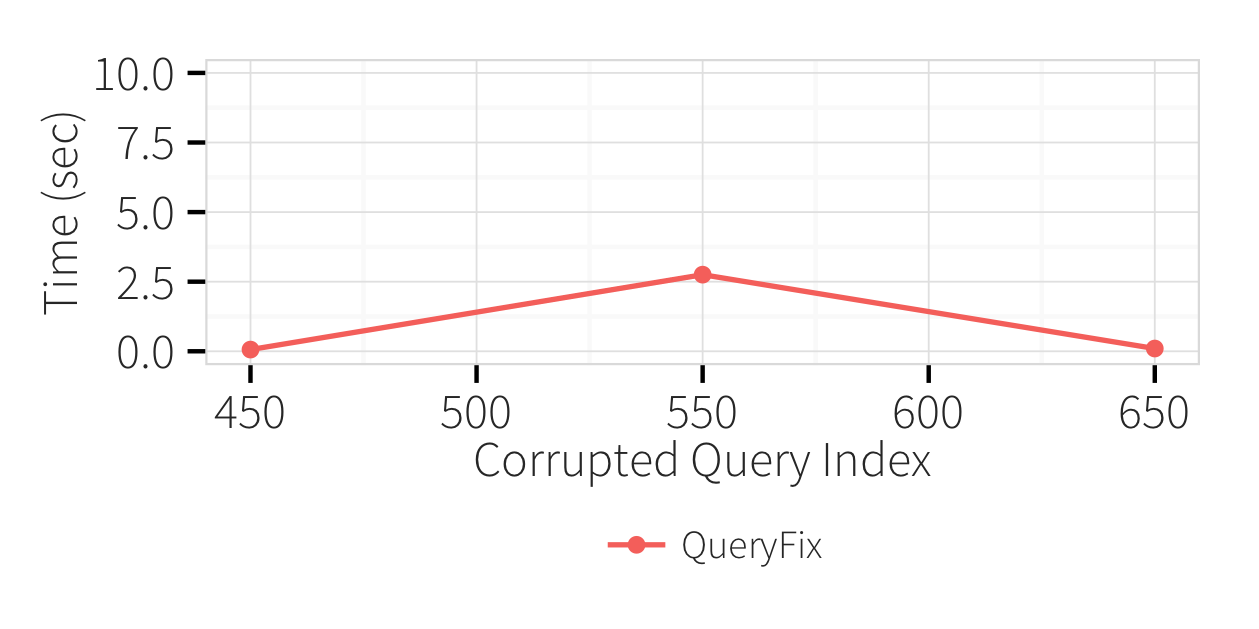
\includegraphics[width = .95\columnwidth]{figures/auction_time}
%   \caption{Performance on AuctionMark Benchmark}
%   \label{f:auctionmark} 
%   \end{subfigure}
%   \caption{Benchmark Performance}
% \end{figure}

\subsection{Preliminaries}

 \begin{figure*}[ht]
    \vspace*{-.1in}
    \centering
    \begin{subfigure}[t]{.49\textwidth}
    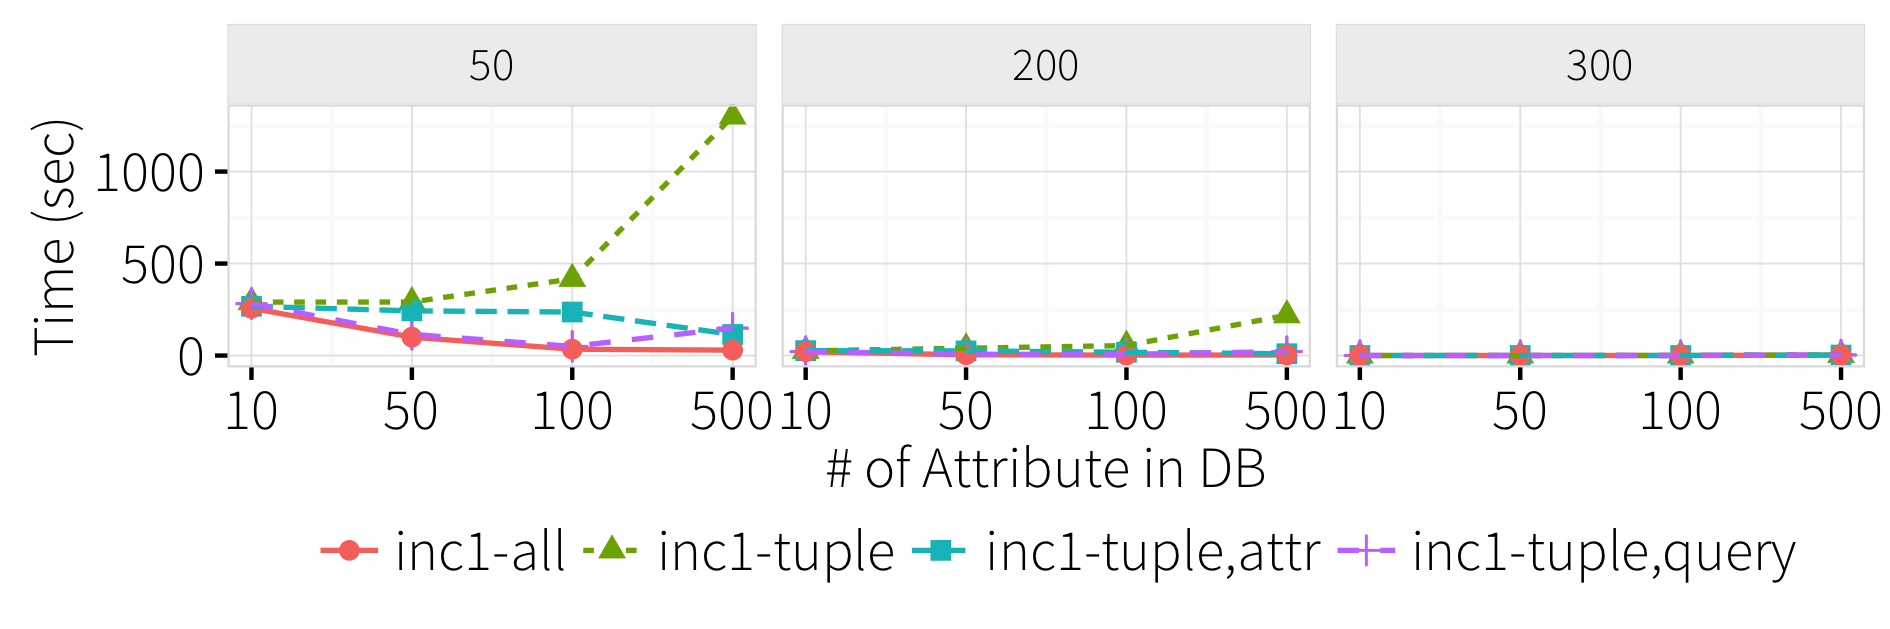
\includegraphics[width = .99\columnwidth]{figures/attr_time}
    \vspace*{-.1in}
    \caption{\# of attributes vs time.}
    \label{f:attr} 
    \end{subfigure}
    \begin{subfigure}[t]{.49\textwidth}
    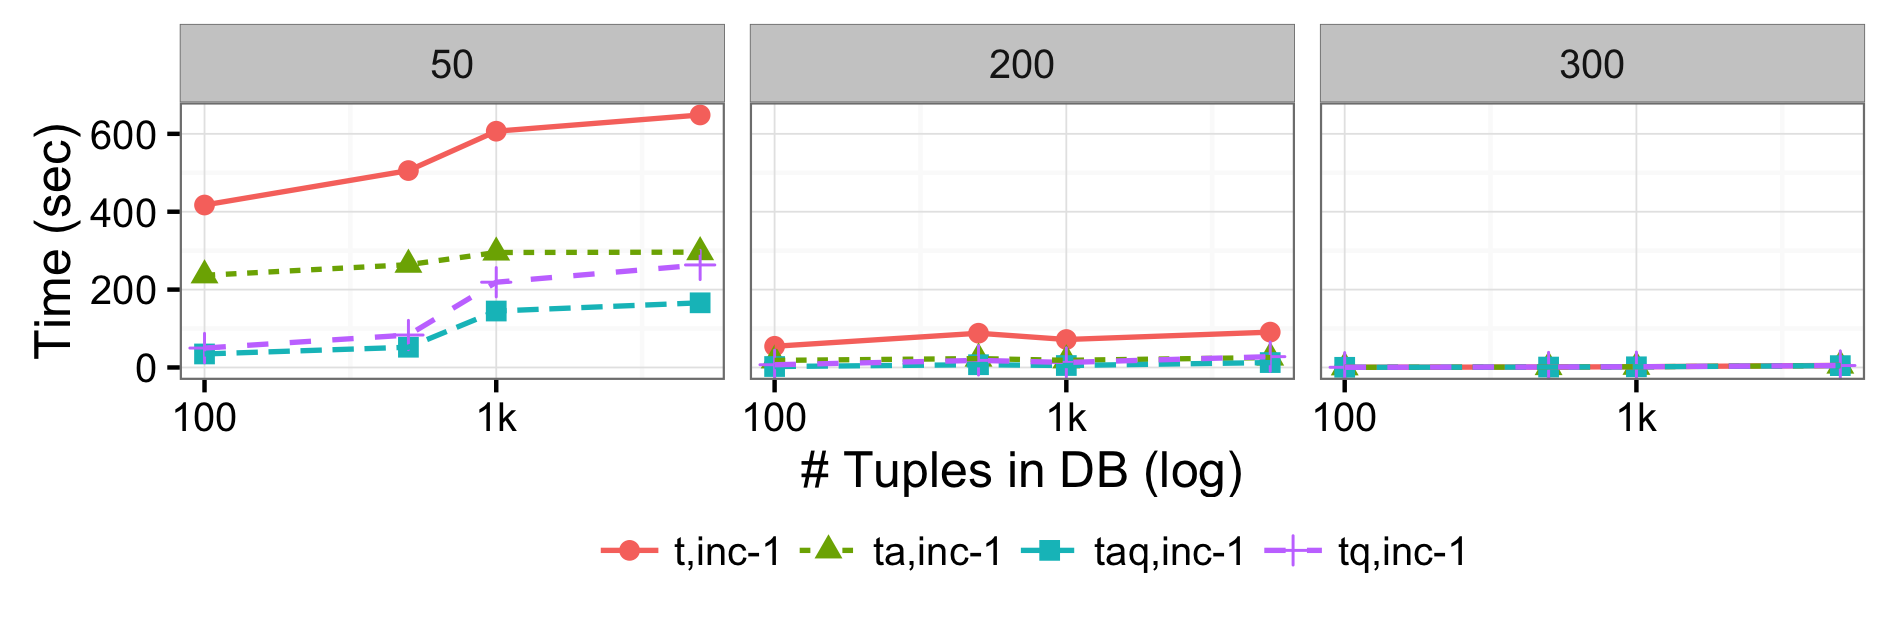
\includegraphics[width = .99\columnwidth]{figures/attr100_time}
    \vspace*{-.1in}
    \caption{Database size vs time ($N_a = 100$)}
    \label{f:attr100} 
    \end{subfigure}
    \vspace*{-.1in}
    \caption{Comparison of optimizations.}
    \vspace*{-.15in}
  \end{figure*}
The following set of experiments are designed to establish the rationale for 
the settings in the subsequent experiments.  
Specifically, we compare different slicing-based optimizations of the basic approach
as the number of queries increases.  
We then evaluate the scalability of the different slicing-based optimizations of the 
incremental approach in the context of a single
corrupted query. We then establish the difficulty of repairing \texttt{UPDATE} 
workloads as compared to other query types. 

\stitle{Multiple Corrupt Queries:}
In this experiment, we compare the basic algorithm ($basic$) against 
each slicing optimization individually($basic-tuple, basic-attr, basic-query$) and all of them together ($basic-all$).  
We use the default settings with $N_D = 1000$ tuples and a sequence of \texttt{UPDATE} queries.
We generate query logs in 5 different sizes $N_q\in \{10, 20, 30, 40, 50\}$ and corrupt 
every tenth query starting from oldest query $q_1$,
up to $q_{41}$.  For example, when the $N_q = {30}$, we corrupt 3 queries: $q_{1,11,21}$. 
We find that the number of queries greatly affects both the scalabality (Figure~\ref{f:multi_time}) 
and the accuracy (Figure~\ref{f:multi_acc}) of the algorithms. Specifically, as the number increases,
the number of possible assignments of the MILP parameters increases exponentially and the solver often takes
longer than our experimental time limit of $1000$ seconds and returns an infeasibility error.  
This is a predominant reason why the accuracy degrades past $30$ queries.  For example, 
when $40$ queries are involved (with $4$ corruptions) 
and we ignore the infeasible executions, the average execution time is $300$ seconds
and the precision and recall are greater than $0.94$.  Unfortunately, with $50$ queries ($5$ corruptions),
all runs exceed the time limit and return infeasibility.

\stitle{Single Corrupt Query:}
In this experiment, we evaluate the efficacy \sys with tuple slicing and incremental optimization
in the special case when one query has been corrupted in a much larger query log. 
We compare \incremental without tuple slicing ($inc_1$) against tuple slicing at 
different batching levels of 1, 2, 8 ($inc_1-tuple; inc_2-tuple, inc_8-tuple$). 
Recall from Section~\ref{sec:incremental} that $inc_k$ parameterizes $k$ consecutive queries in each batch until a repair is found.
Figure~\ref{f:singlequeryinc_time} highlights the scalability limitation of the incremental 
algorithm without tuple-slicing: with 50 queries $inc_1$  easily exceeds the 1000s limit.   
The tuple-slicing scales significantly better (nearly $200\times$ faster), however
the accuracy severely degrades when $k>1$.  
The primary reason is because of infeasibility errors---the MILP problem is much harder, and fails to find a repair.  
This is highlighted by the symmetry between the precision and recall curves.  
A secondary reason is beause the refinement step of  tuple slicing may not generate a fully correct repair and generalize incorrectly.
This is why the precision curve is lower than the recall curve for $inc_8-tuple$.




\stitle{Query Type:}\label{sec:indelup}
Our final preliminary experiment evaluates the incremental algorithm with tuple slicing optimization 
($inc_1-tuple$) on \texttt{INSERT}, \texttt{DELETE}, or \texttt{UPDATE}-only workloads.
We increase the number of queries from $1$ to $200$ and corrupt the oldest query in the log.  
Figure~\ref{f:indelup_time} shows that while the cost of repairing \texttt{INSERT} workloads
remains relatively constant, the cost for \texttt{DELETE}-only and \texttt{UPDATE}-only workloads increase as 
the corruption happens earlier in the query log---and a much faster rate for \texttt{UPDATE} queries.
The F1 score for all settings is nearly 1 (Figure~\ref{f:indelup_acc}).

\smallskip
{\it Takeaways: we find that \texttt{basic}, even with slicing optimizations,
has severe scalability limitations due to the large number of undetermined values -- this is not surprising
since MILP constraint solving is a known NP-hard problem.
In contrast, the incremental algorithms can scale to larger query log sizes, however only a batch size of $k=1$ can retain high repair quality.
Furthermore, we show that \texttt{UPDATE}-only workloads are significantly more expensive to repair than other query types. 
Based on these results, we focus on the incremental algorithm $inc_1$ and the more difficult \texttt{UPDATE}-only workloads.
%Based on the result, we consider incremental algorithm at batching level 1 with tuple slicing optimization ($inc_1-tuple$) as default setting in the rest of the experiment. In addition, we only consider \texttt{UPDATE}-only workload in synthetic experiments in Section~\ref{sec:experiments:synth}. 
}

\subsection{Synthetic Incremental Experiments}
\label{sec:experiments:synth}
%We now perform a detailed evaluation of the incremental algorithm (batching level 1).
We divide these experiments into two groups: the first evaluates the different slicing optimizations under different settings; 
the latter algorithm and varies workload and dataset parameters.
Note that omit accuracy figures when the F1-score is $\ge 0.99$.

\noindent\textbf{Comparing Optimizations}

\emph{Varying \# Attributes:}
We first evaluate \sys and its optimizations by increasing the number of attribute ($N_a \in [10, 500]$) with $N_D = 100$.
As shown in Figure~\ref{f:attr}, when the number of attribute in a table is small (e.g., $N_a=10$) all algorithms appear identical. 
However, increasing the number of attribute exhibits a larger benefit for query and attribute slicing (up to $6.8\times$ reduction compared to tuple-slicing).
When the table is wide ($N_a = 500$), applying all optimizations ($inc_1-all$) is $40\times$ faster than \emph{tuple-slicing} alone.  

\emph{Database Size:} 
We vary the database size ($N_D \in [100,5000]$) with a large number of attributes ($N_a = 100$).
We fix the number of complaints by decreasing the query selectivity in proportion to $N_D$'s increase---the specific mechanism to do so does not affect the findings.
Figure~\ref{f:attr100} shows that the costs are relatively flat until the corruption occurs in an old query ($q_{50}$).  
In addition, we find that the cost is highly correlated with the number of candidate queries that are encoded in the MILP problem.
The increase in cost despite tuple-slicing is due to the increasing number of candidate queries in the system; 
we believe this increasing trend is due to the solver's ability to prune constraints that correspond to queries that clearly will not affect the complaint set---an implicit form of query slicing.  
Applying attribute-slicing supercedes this implicit optimization and results in a flat curve, 
while query-slicing explicitly reduces the number of candidate queries in proportion with the database size, and leads to the increasing trend.
Ultimately, combining all three optimizations improves the latency over tuple-slicing by $2\times$ in the worst case, and up to $4\times$ in the best case.
%We find that the large number of attributes allows query and attribute slicing to have a large effect on the performance.
% The increase in cost despite the tuple-slicing optimization is an artifact of increasing $V_d$, which increases the space of possible value assignment for each undetermined variable.
% In fact, the number of constraints remains constant as the database increases, illustrating tuple-slicing's effectiveness.

% \ewu{why does the cost increase while the next experiment is flat??}
% The large number of attributes in the schema enables the query and attribute optimizations to have a large effect.
% \xlw{
% In Figure~\ref{f:attr100}, we see that the time cost grows as database size increases for approach with only \emph{tuple-slicing} optimization. This is because we increase the range $[0, V_d]$ of each attribute in order to keep the same query selectivity as database size increases. Thus, the searching space of the problem also grows and so does the execution time. However, \emph{attribute-slicing} helps reducing the impact as it only encodes relevant attributes. As a result, we observe a much slower time cost growing rate for algorithm with \emph{attribute-slicing} optimization. Overall, we observe that approach with all optimizations ($inc_1-all$)
% shows more than $50\%$ efficiency gain over with only tuple-slicing optimization as the database size increases. Note that the impact of attribute ranges $[0, V_d]$ also relevant to number of attribute in the table, it would not increase the searching space (or time cost) as significant as for problems with fewer attributes (e.g., 10). 
% }

% Motivated by our preliminary results, we focus on \texttt{UPDATE}-only query logs with a single corruption with
% $10$ attributes and $1k$ attributes in the table. As the performance of \sys with different optimizations appears 
% identical when $N_a = 10$, we will only show results of \sys with tuple slicing optimization in the rest of the 
% experiments. 
  \begin{figure*}[ht]
    \hspace*{-.1in}
    \centering
     \begin{subfigure}[t]{.33\textwidth}
      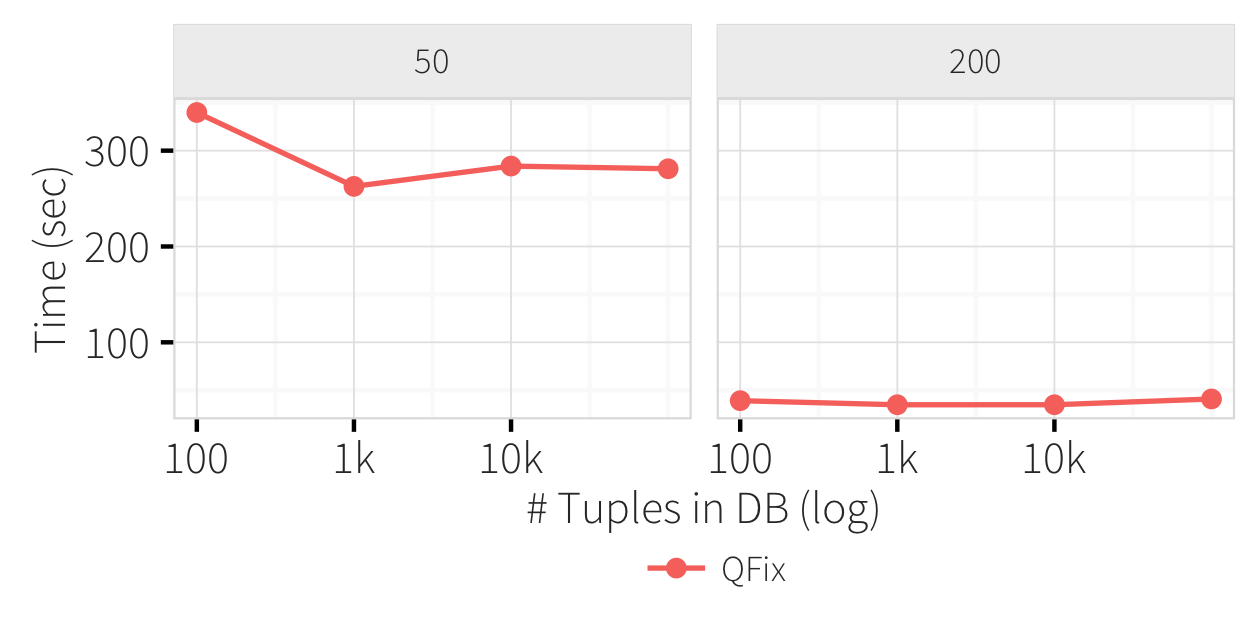
\includegraphics[width = .99\columnwidth]{figures/dbsize_time}
      \vspace*{-.25in}
      \caption{Database size vs time.}
      \label{f:dbsize_time} 
    \end{subfigure}
    \begin{subfigure}[t]{.33\textwidth}
      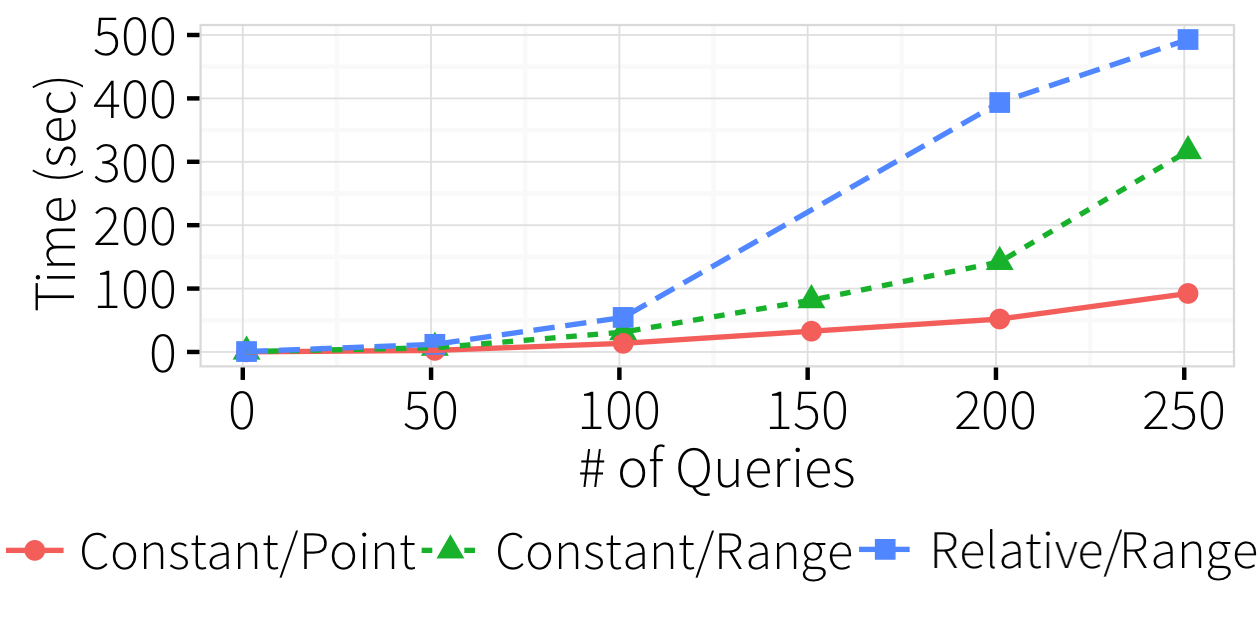
\includegraphics[width = .99\columnwidth]{figures/pointrelv_time}
      \vspace*{-.25in}
      \caption{Performance of diff. query clause types.}
      \label{f:qidx_time} 
    \end{subfigure}
    \begin{subfigure}[t]{.33\textwidth}
      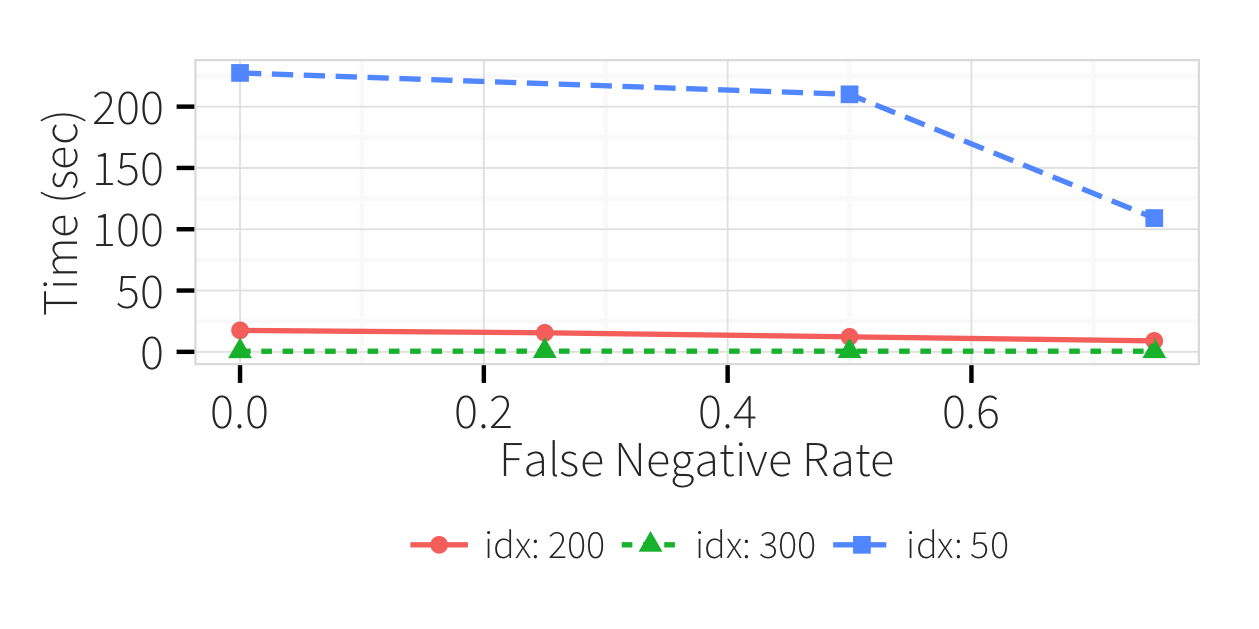
\includegraphics[width = .99\columnwidth]{figures/noise_fn_time}
      \vspace*{-.25in}
      \caption{False negatives vs time.}
      \label{f:falsenegative_time} 
    \end{subfigure} 
    \\
    \hspace*{-.1in}
    \vspace*{.2in}
    \begin{subfigure}[t]{.33\textwidth}
      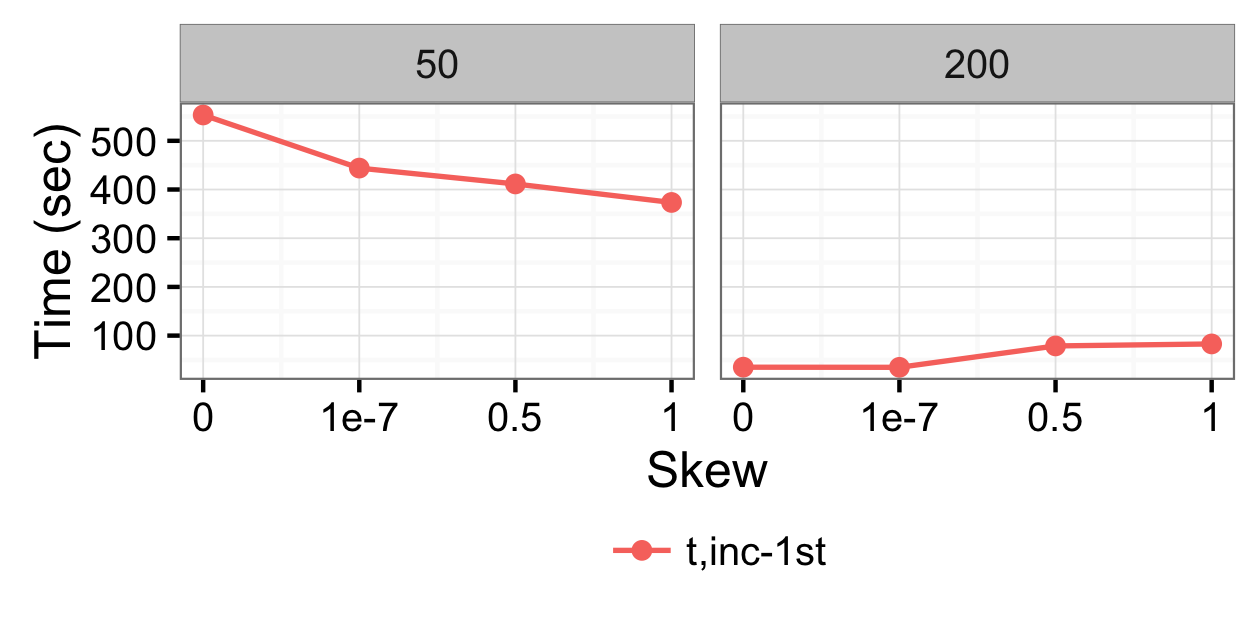
\includegraphics[width = .99\columnwidth]{figures/skew_time}
      \vspace*{-.25in}
      \caption{Skew vs time.}
      \label{f:skew_time} 
    \end{subfigure}
    \begin{subfigure}[t]{.33\textwidth}
      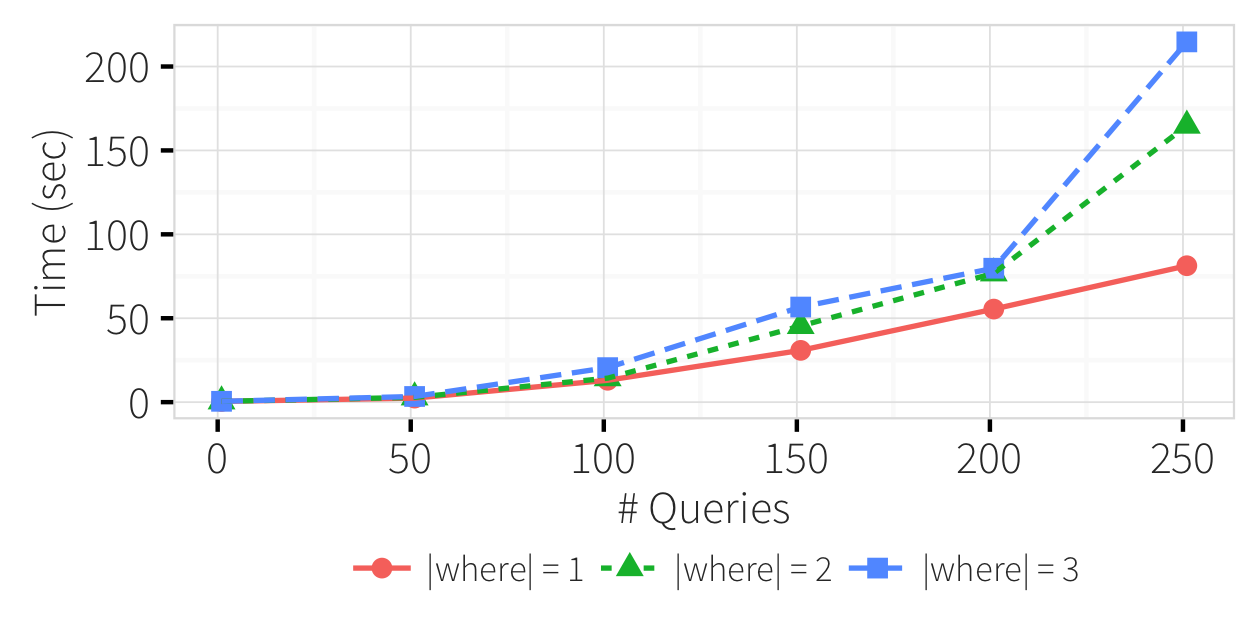
\includegraphics[width = .99\columnwidth]{figures/where_time}
      \vspace*{-.25in}
      \caption{Query dimensionality vs time.}
      \label{f:where_time} 
    \end{subfigure}
    \begin{subfigure}[t]{.33\textwidth}
      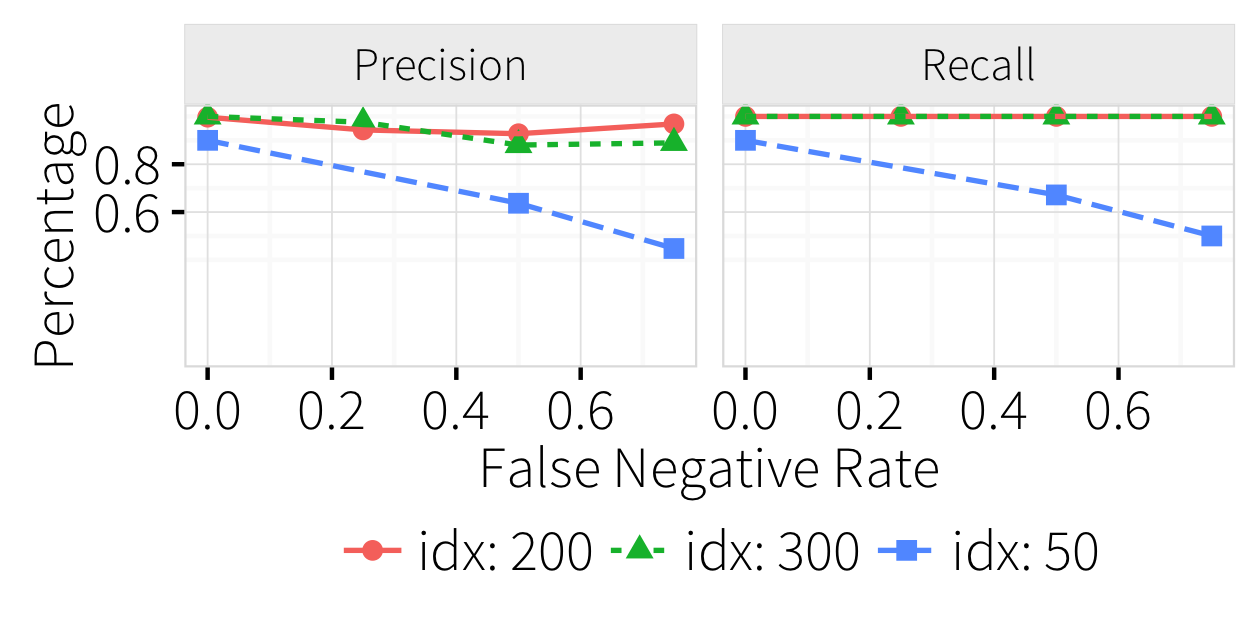
\includegraphics[width = .99\columnwidth]{figures/noise_fn_acc}
      \vspace*{-.25in}
      \caption{False negatives vs accuracy.}
      \label{f:falsenegative_acc} 
    \end{subfigure}
    \vspace*{-.25in}
    \caption{Sensitivity to data and workload factors. }
    \vspace*{-.15in}
  \end{figure*}


\noindent\textbf{Sensitivity to Data and Workload Factors}

The following set of synthetic experiments focus on a single \sys setting---incremental with tuple-slicing---and
individually vary numerous database and workload parameters in order to tease apart the algorithm performance.  
These include factors such as query complexity, log size $N_q$, database size $N_D$ and the skew of the query predicates.
We focus on a narrow table setting that contains $N_a = 10$ attributes, and a single corrupt query in the query log.


% \iffalse 
%   \stitle{Scalability - Log Size:}
%   Figures~\ref{f:logsize_time} and~\ref{f:logsize_acc} increase the query log size (each subplot) between $50, 100, 500$ and $1000$.
%   We compared the baseline $\sys_{t,inc}^{1st}$ with addition attribute, query or both slicing optimizations.
%   For readibility purposes, we have normalized the x-axis to show the distance of the corrupted query from the most recent query in the log
%   (e.g., $x=50$ denotes that $q_{N-50}$ was corrupted).
%   As expectied, the cost increases as the corruption is older in the query log since more queries need to be tested before the
%   true corruption is encountered.  There algorithms all execute at roughly the same performance, though there is a slight advantage to
%   using the query-slicing optimization. The optimization reduces the time to linearize the query log by roughly $20\%$, however
%   the CPLEX solver time contributes to over half the total time so the improvement is difficult to see.
%   All algorithms exhibit near perfect F1-scores.
% \fi


\emph{Database Size:}
Figure~\ref{f:dbsize_time} varies the database size ($N_D \in [100, 100k]$), and fixes query output cardinality and complaint set size in the same way as the previous scalability experiment.
In contrast to the previous experiment, the scalabality curve is nearly flat for both corruption query indices.
The reason is because the solver's implicit pruning optimization is less effective when there are only $10$ attributes: Every query is likely to touch an attribute that affects the complaint set.
We verified this by applyng query-slicing to the same setting, and found that significant less amount of queries were pruned compared to previous experiment.
The more recent corruption at $q_{200}$ is executed within 40 seconds even as the database size increases, with a perfect F1-score. 
When the corruption is old ($q_{50}$), the performance is more variable at smaller database sizes due to the randomness in the data and query generator.
This leads to more variability in the size of the resulting complaint set, which increases the size and difficulty of the encoded problem, and leads to the spike in average latency at small database sizes.

% due to the smaller number of attributes, which reduces the effect of increasding $V_d$.  
% Recall that the size of the MILP problem increases multiplicatively with the number of tuples and attributes.  
% Thus reducing number of attributes in combination with tuple-slicing effectively contrains the size of the MILP problem.
% The more recent corruption at $q_{200}$ is executed in nearly constant time as the database size increases, with a perfect F1-score. 
% The performance is more variable at smaller database sizes due to variability in the true query selectivity due to randomness in the data and query generator.
% This leads to more variability in the size of the resulting complaint set, which increases the size of the encoded problem.
% Since the solver scales exponentially with the problem size, this leads to the performance spike when the database is small.


\emph{Query Clause Type: }
So far, we have focused on \texttt{UPDATE} queries with constant set clauses and range predicates.  
Figure~\ref{f:qidx_time} individually varies each clause and compares against {\it Constant/Point} and {\it Relative/Range} queries. 
The x-axis varies the index of the corrupted query between $q_1$ and $q_{249}$.
We find that point predicates and constant set clauses are easier to solve than range predicates and relative set clauses, respectively.
The reason for the former pair is because range predicates double the number of undetermined variables as compared to point queries.  
In addition, point queries are on key attributes, thus further reduces the possible search space.  
We believe the latter pair is because the constant set clauses break the causal relationship between input and output records for the overwritten values.
This both simplifies the difficulty of the constraint problem, and reduces the total number of constraints.

% constant set clauses disconnect tuple values from query to query whereas relative set clauses maintain this connection. Thus, the searching space for the relative set clauses is often bigger than the constant one; 
% 2. since relative set clauses maintain the tuple value connection, their complaint set sizes are normally larger than constant set clauses for the same corrupt index: In relative set clauses, incorrectness always inherits from previous database state and could infects other tuples, however, this is less likely to happen for constant set clauses.}

\emph{Query Predicate Dimensionality:}
Figure~\ref{f:where_time} varies the dimensionality of the update queries by increasing the number of predicates in the \texttt{WHERE} clause, while keeping the query cardinality constant.
The cost increases with the dimensionality because each additional predicate is translated into a new set of constraints and undetermined variables, increasing the problem complexity.
% From Figure~\ref{f:where_time}, we found that more predicates increases the cost in solving a problem. 
% This is expected as when there are more predicates, the number of constraints and variables in the MILP problem also increase, which further increase the problem complexity.

%We find that the performance improves as the number of predicates increases.
%This counter-intuitive result is due to the reduction in the complaint set size as the complexity increases. 
%Again, we omit the accuracy result as \sys exhibit above 0.996 average F1 score in all settings. 


\emph{Skew:} We now study the effects of attribute skew on the algorithms.
We increase the skew parameter from $0$ (uniform) to $1$ (nearly every attribute is $A_0$) 
and find a reduction in latency (Figure~\ref{f:skew_time}).
We believe the reason is because increasing the skew focuses the query predicates over a smaller set of logical attributes, 
and increases the number of constraints placed on each of the logical attributes used in the query log.  
Each of these constraints reduces the search space of allowable values for that attribute, and thus simplifies the MILP problem.
This result suggests that \sys may be well suited for many transaction systems that naturally exhibit query skew.
Note that the overall number of constraints in the problem is the same, only their distribution over the query attributes has changed.


% \xlw{
% Higher skewness factor increases the update frequency of certain attributes, which further increases the number of constraints on these attributes. With more constraints, the searching space get reduced and thus the problem becomes easier to solve. The update frequency of an attribute is a combined result of the skewness factor and the number of queries in the problem: one would only observe the (frequency) difference when there are enough number of queries. 
% Thus
% we observe a clear decreasing trend in Figure~\ref{f:skew_time} as we increase the skewness factor on corrupt index equals to $50$ ($250$ queries from the most recent one). 
% However, when the corruption is more recent (corrupt index equals to $200$, $50$ queries to the most recent one), this trend \sout{can be hardly seen} is less significant.
% }

% 
% Our hypothesis is that higher skew results in a larger number of relevant queries, thus limiting the effectiveness of query slicing.
% In addition, recall that each query sets all tuples within the same range to the same value.  
% Since increasing the skew makes it more likely that both the \texttt{SET} and \texttt{WHERE} clauses reference the same attributes,
% it causes the tuples to cluster around the values, thus increasing the selectivity of the queries.
% This results in a larger complaint set, which 
% 
% with high skew, each query is more likely to modify the same tuples, thus increasing the number of
% 
% We generate query log at 4 different skewness levels from uniform to 
% super skewed with $s = 0, 1e-7, 0.5, 1$. As we can see as query log
% is more skewed, the execution time for solving same amount of queries 
% increase. This is also due to the fact that increasing skewness also
% increase the query dependency, which, in turn, increase the searching
% space in the MILP problem.


\emph{Incomplete Complaint Sets:}
Our final experiment (Figures~\ref{f:falsenegative_time} and~\ref{f:falsenegative_acc}) varies the fase positive rate in incomplete complaint sets.
We increase the rate from $0$ ($0\%$ missing in the complaint set) to $.75$ ($75\%$ are missing).  
We find that reducing the size of the submitted complaint set naturally improves the repair performance,
however the repair quality, both precision and recall in Figure~\ref{f:falsenegative_acc}, may suffer if the corruption occured in a very old query. 
This is expected because \sys targets reported complaints, thus unreported complaints may easily be missed and lead to low recall.
In addition, despite the refinement step of tuple-slicing, the repair may over generalize and ``fix'' the wrong records, leading to low precision.
%\ewu{Can we hand look at some of the results and make a qualitative description of if the results are "good" or not?}
%   \begin{figure}[h!]
%     \centering
%     \begin{subfigure}[t]{\columnwidth}
%     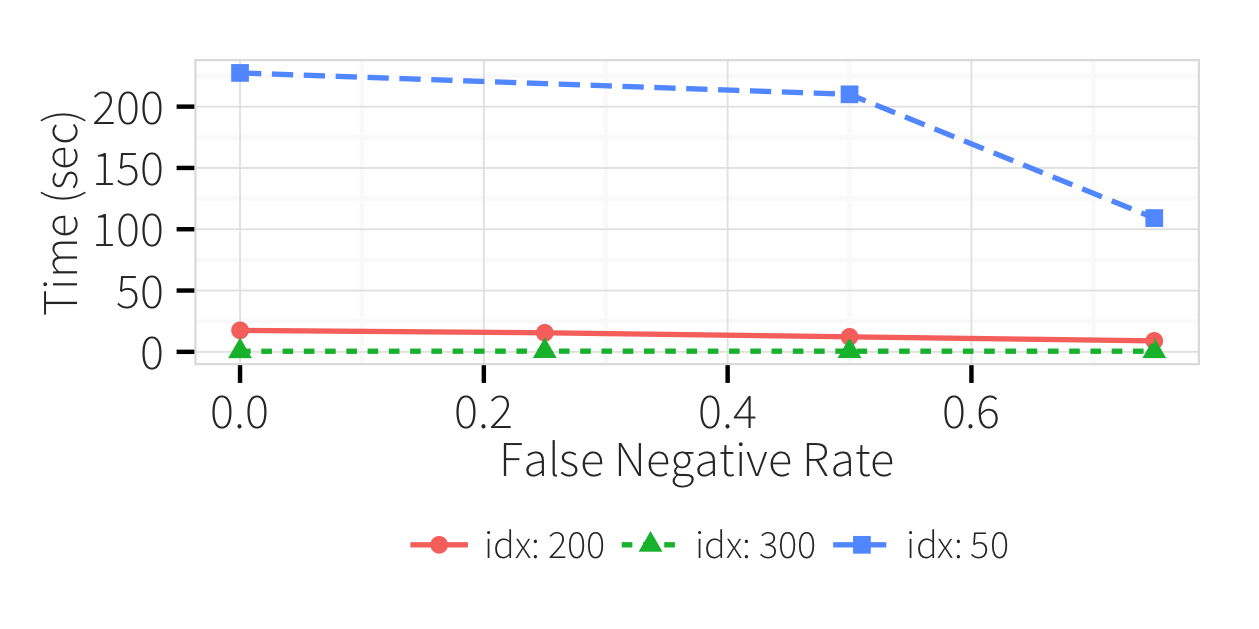
\includegraphics[width = .9\columnwidth]{figures/noise_fn_time}
%     \caption{Time vs Incomplete Complaint Size}
%     \label{f:falsenegative_time} 
%     \end{subfigure}
%     \begin{subfigure}[t]{\columnwidth}
%     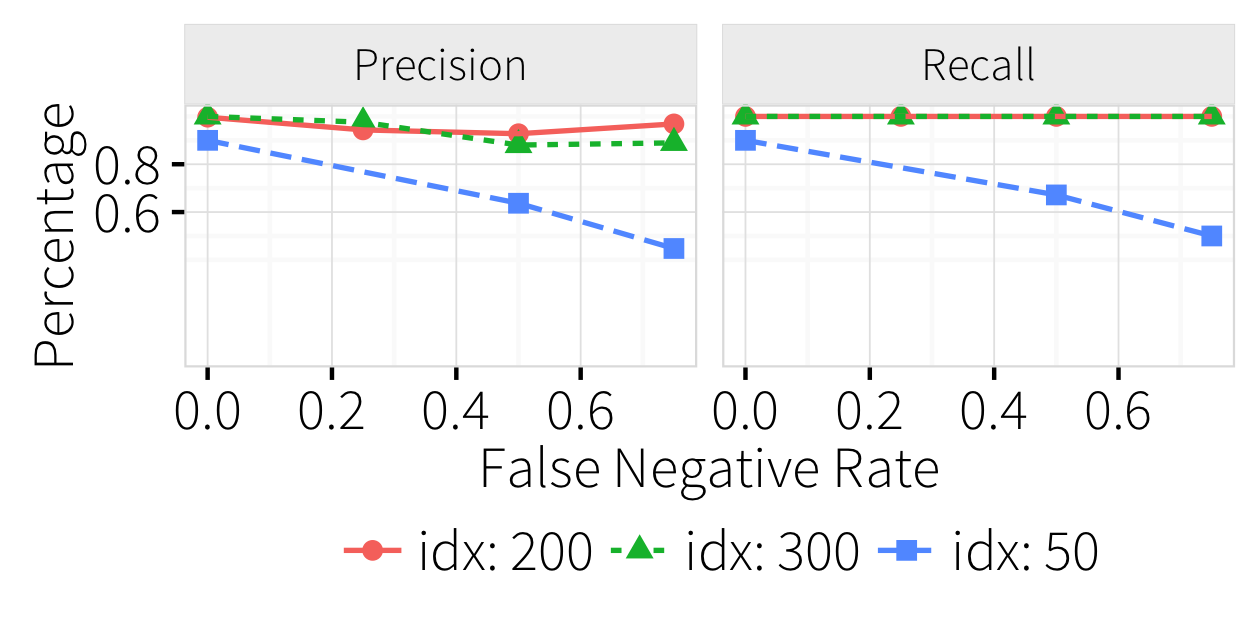
\includegraphics[width = .9\columnwidth]{figures/noise_fn_acc}
%     \caption{F1-score vs Incomplete Complaint Size}
%     \label{f:falsenegative_acc} 
%     \end{subfigure}
%     \label{f:falsenegative}
%     \caption{Incomplete Complaint Experiments}
%   \end{figure}
% 
\smallskip
\textit{Takeaways: we find that the performance of the different repair algorithm 
heavily depends on the property of the datasets and queries. Attribute and query slicing show significant gain for 
datasets with large number of attributes and \sys is able to solve hard problems
(with ~$200$ \texttt{UPDATE}-only queries) in seconds or minutes---particular if the error is recent. }

\subsection{Benchmarks}
\label{sec:experiments:benchmark}

Figure~\ref{f:tpcctatp} plots the performance of the incremental algorithm using tuple-slicing on the TPC-C and TATP benchmark applications.  
The key reason is that each query affects a small set of records and leads to a very small complaint set---$1$ or $2$ on average.
In addition, tuple and query slicing can aggressively reduce the total number of constraints to a very small number---often less than $100$ in total.
Furthermore for TPC-C, the queries are predominantly \texttt{INSERT} queries, which \sys can solve within milliseconds.

{\it Takeaway: many workloads in practice are dominated by \texttt{INSERT} and point \texttt{UPDATE} queries.  
  In these settings, \sys is very effective at reducing the number of constraints and can derive repairs with near-interactive latencies.}
\begin{figure}[h]
\centering
  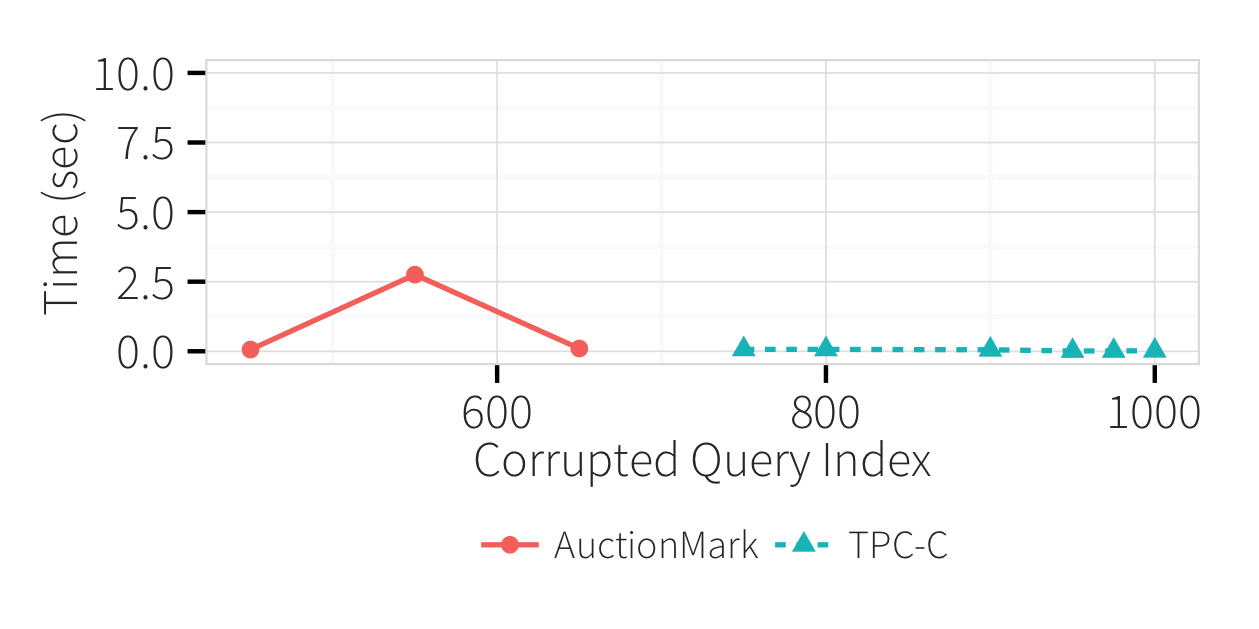
\includegraphics[width = .75\columnwidth]{figures/benchmark_time}
  \vspace*{-.2in}
  \caption{Performance on benchmarks}
  \label{f:tpcctatp} 
  \vspace*{-.1in}
\end{figure}

\iffalse  
  \begin{figure*}[h]
    \centering
    \begin{subfigure}[t]{.3\textwidth}
      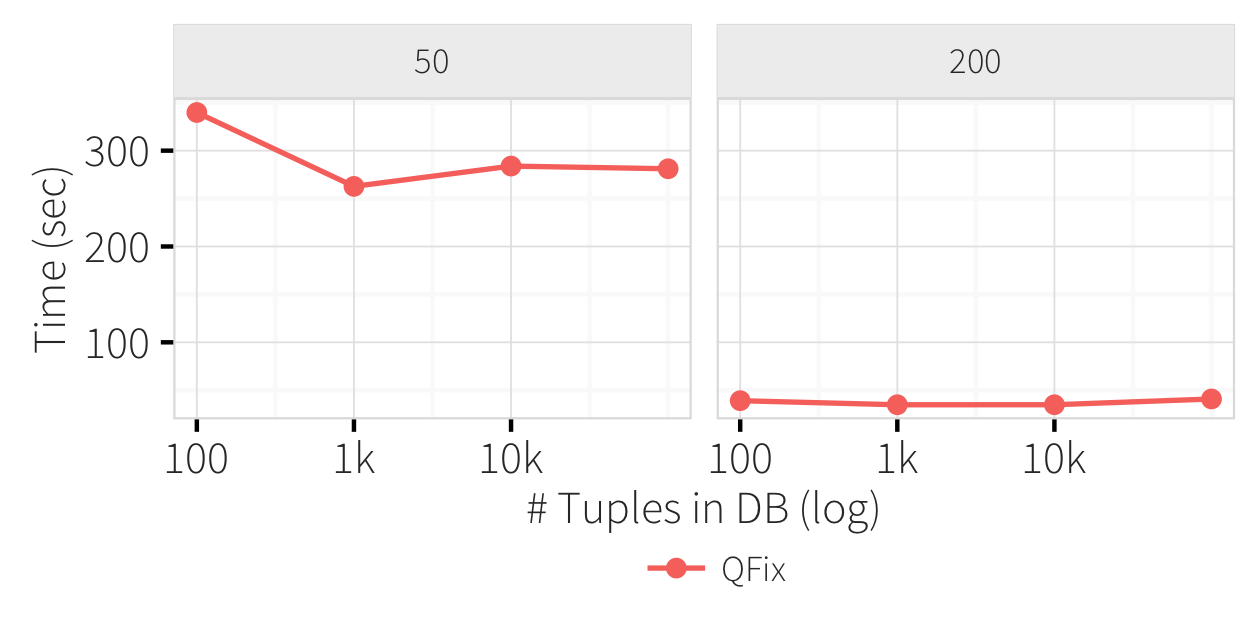
\includegraphics[width = .99\columnwidth]{figures/dbsize_time}
      \vspace*{-.1in}
      \caption{Database Size.}
      \label{f:dbsize_time} 
    \end{subfigure}
        \begin{subfigure}[t]{.3\textwidth}
      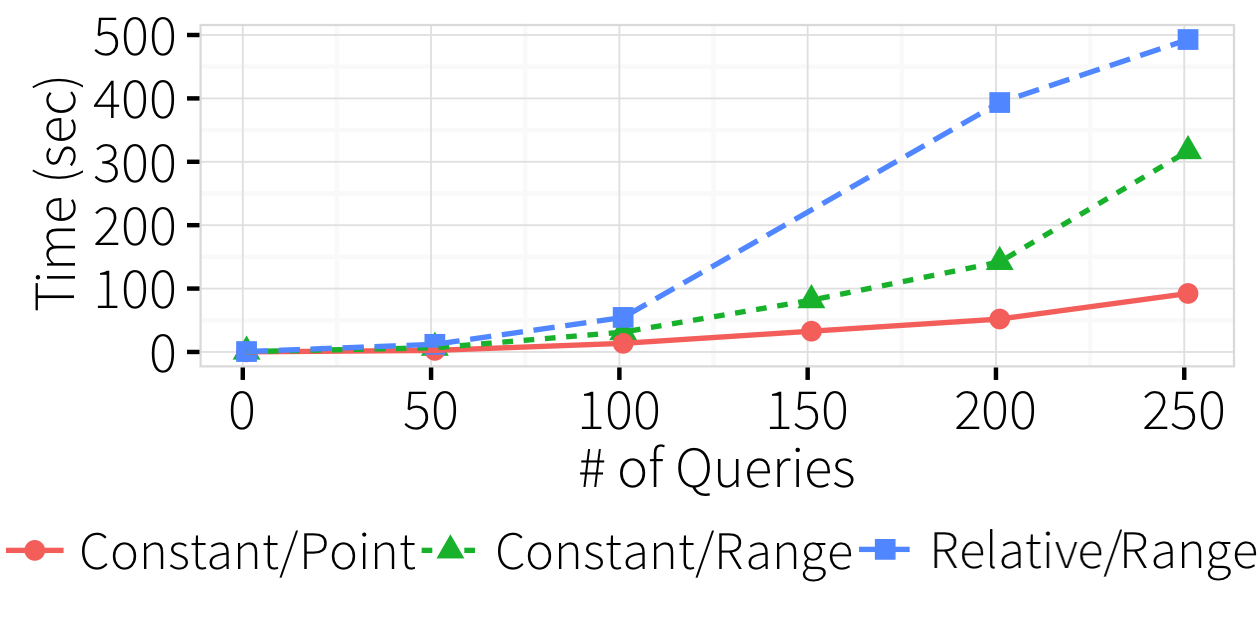
\includegraphics[width = .99\columnwidth]{figures/pointrelv_time}
      \vspace*{-.1in}
      \caption{Query Complexity (Query Type).}
      \label{f:qidx_time} 
    \end{subfigure}
    \begin{subfigure}[t]{.3\textwidth}
      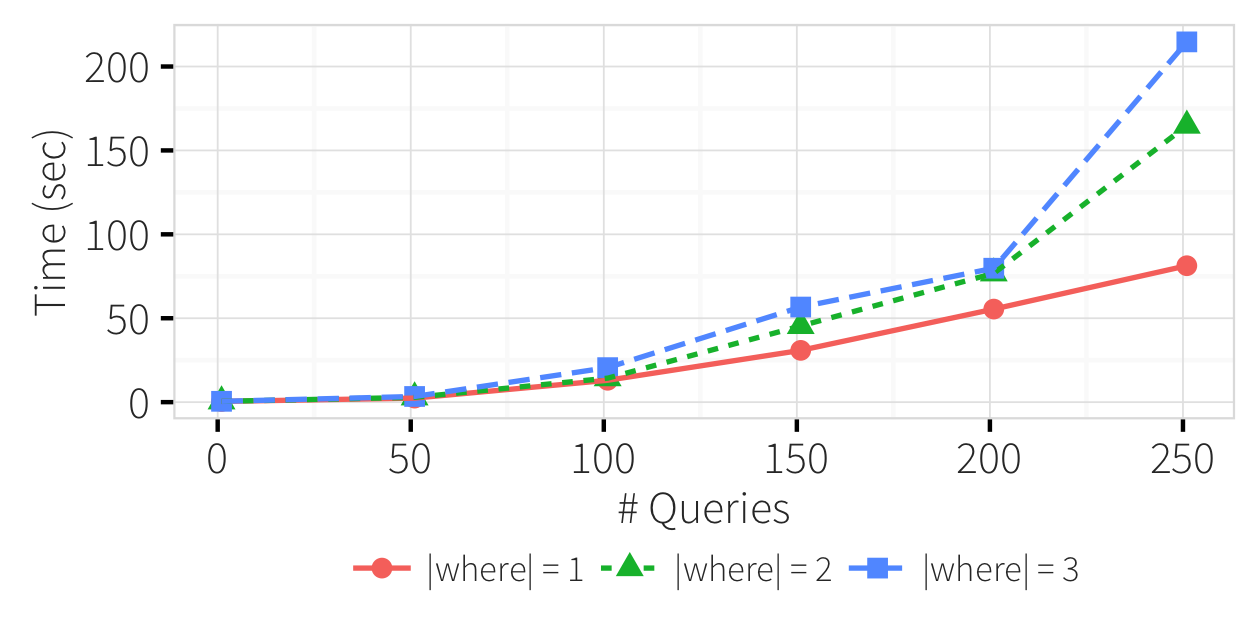
\includegraphics[width = .99\columnwidth]{figures/where_time}
      \vspace*{-.1in}
      \caption{Query Complexity (Where Size).}
      \label{f:where_time} 
    \end{subfigure}
    \\
    \begin{subfigure}[t]{.3\textwidth}
      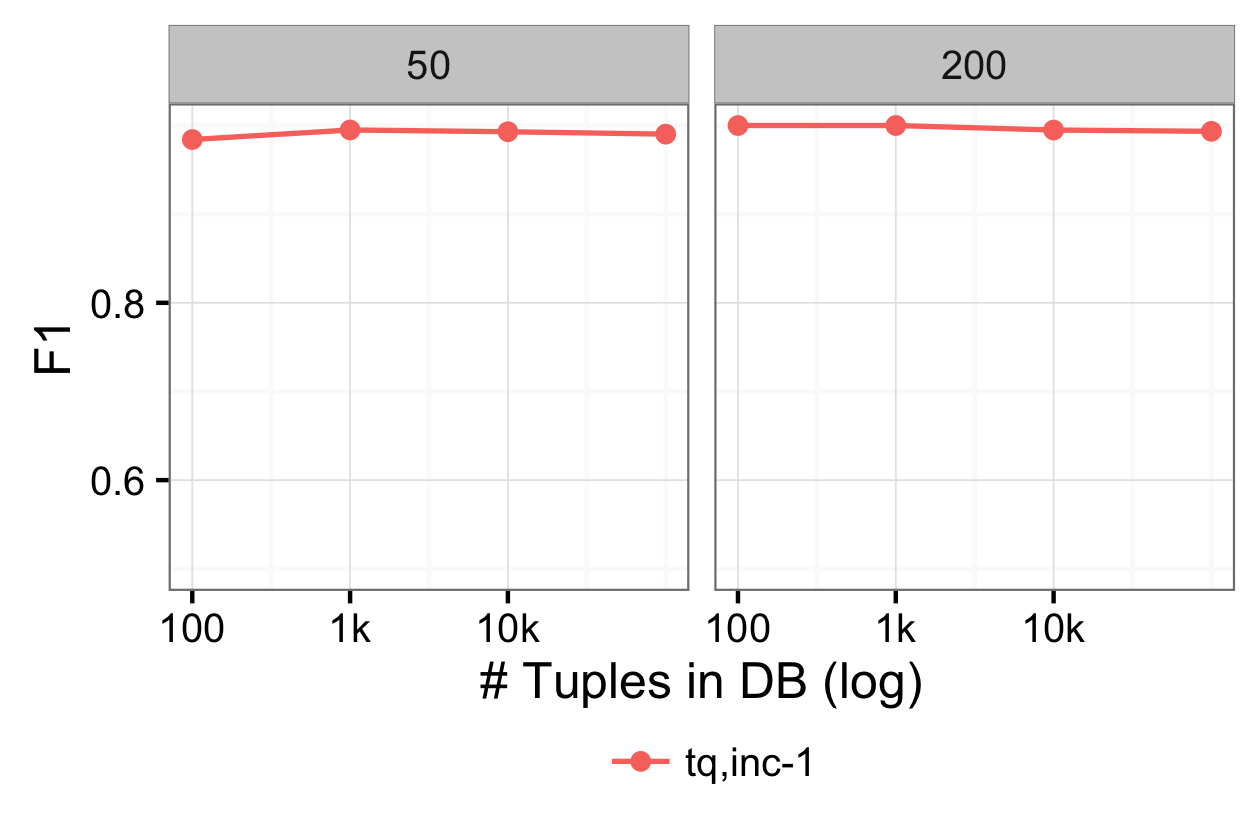
\includegraphics[width = .99\columnwidth]{figures/dbsize_acc}
      \vspace*{-.1in}
      \caption{Database Size vs F1-score. }
      \label{f:dbsize_acc} 
    \end{subfigure}
        \begin{subfigure}[t]{.3\textwidth}
      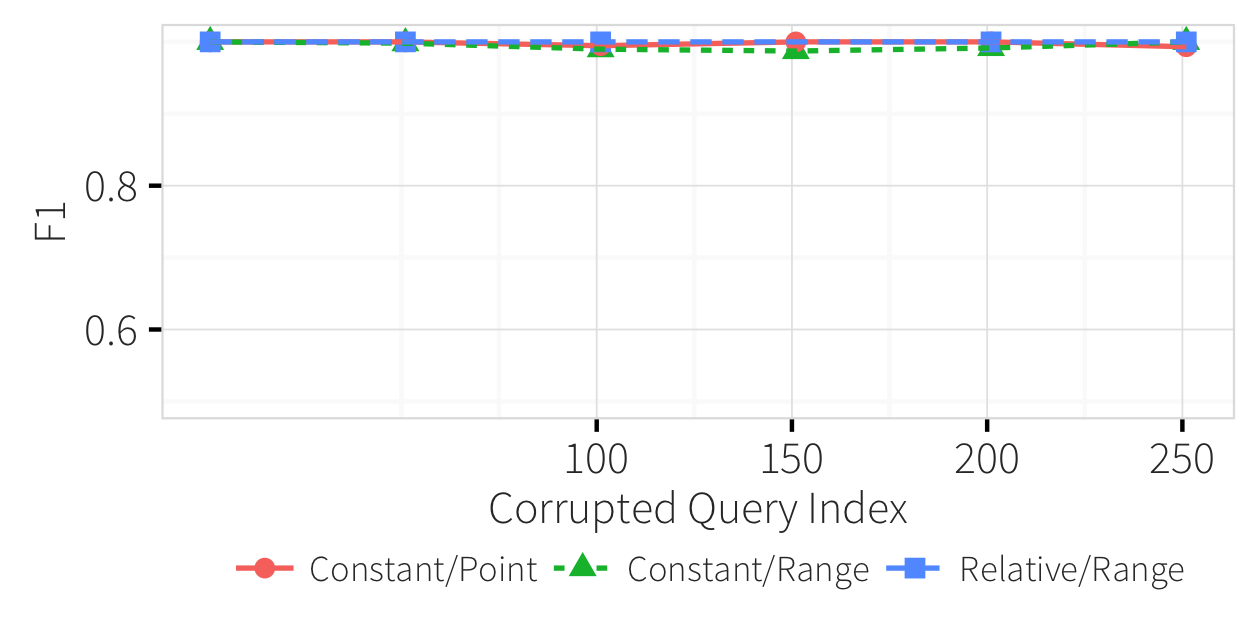
\includegraphics[width = .99\columnwidth]{figures/pointrelv_acc}
      \vspace*{-.1in}
      \caption{Query Complexity (Query Type) vs F1-score.}
      \label{f:qidx_acc} 
    \end{subfigure}
    \begin{subfigure}[t]{.3\textwidth}
      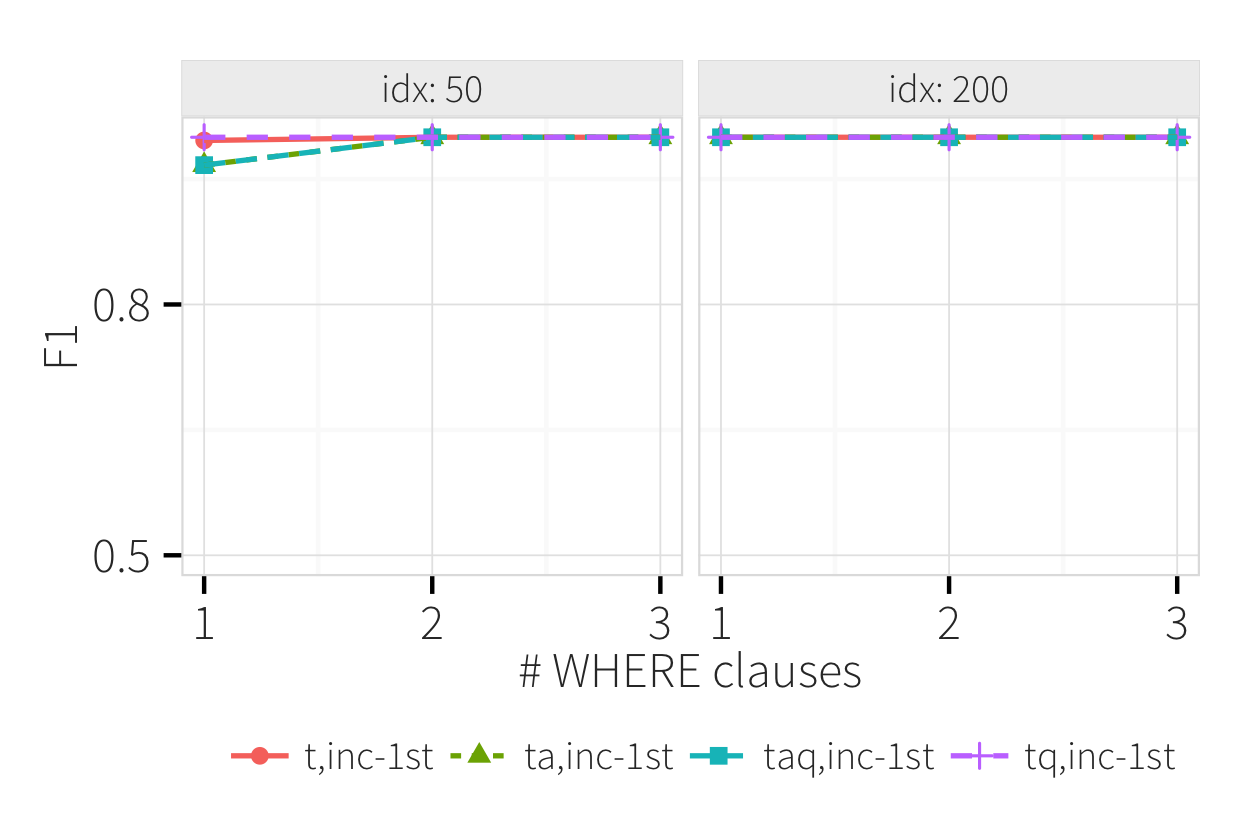
\includegraphics[width = .99\columnwidth]{figures/where_acc}
      \vspace*{-.1in}
      \caption{Query Complexity (Where Size) vs F1-score.}
      \label{f:where_acc} 
    \end{subfigure}
    
    \caption{Scalability Experiments (Performance)}
  \end{figure*}
\fi

